\documentclass[tikz]{standalone}
\usepackage{tikz}
\usetikzlibrary{calc}
\usetikzlibrary{positioning}
\usetikzlibrary{fit}
\usetikzlibrary{backgrounds}

\definecolor{lightGreen}{HTML}{d5e8d4}
\definecolor{lightYellow}{HTML}{fff2cc}
\definecolor{lightGray}{HTML}{f5f5f5}
\definecolor{lightRed}{HTML}{ff9999}
\definecolor{lightBlue}{HTML}{d5e5fc}
\definecolor{lightCyan}{HTML}{a7dfe3}
\pgfdeclarelayer{main_bg}
\pgfdeclarelayer{back_bg}
\pgfsetlayers{main_bg,back_bg,main}

\newcommand{\metarect}[7]{
    \begin{scope}
        \node (#1) [rectangle, draw, text width=\rectWidth, minimum width=\rectWidth, minimum height=\rectHeight, #7] {};
        \node (#1_upper) [rectangle, draw, fill=#6, text width=\rectWidth, minimum width=\rectWidth, minimum height=\rectHeight*0.5, below=0.0pt of #1.north, anchor=north] {#2};
        \node (#1_middle) [rectangle, draw, fill=white, font=\tiny, text width=\rectWidth, minimum width=\rectWidth, minimum height=\rectHeight*0.25, below=-\the\pgflinewidth of #1_upper] {#3};
        \node (#1_bleft) [rectangle, draw, fill=white, font=\tiny, text width=\rectWidth*0.35, minimum width=\rectWidth*0.35, minimum height=\rectHeight*0.25, below=-\the\pgflinewidth of #1_middle.south west, anchor=north west] {#4};
        \node (#1_bright) [rectangle, draw, fill=white, font=\tiny, text width=\rectWidth*0.65, minimum width=\rectWidth*0.65, minimum height=\rectHeight*0.25, right=-\the\pgflinewidth of #1_bleft] {#5};
    \end{scope}
}

\newcommand{\metarectvec}[5]{
    \begin{scope}
        \node (#1) [draw, rectangle, text width=\rectWidth, minimum width=\rectWidth, minimum height=\rectHeight*0.25, #5] {};
        \node (#1_left) [draw, rectangle, fill=#4, font=\footnotesize, text width=\rectWidth*0.4, minimum width=\rectWidth*0.4, minimum height=\rectHeight*0.25, below=0.0pt of #1.north west, anchor=north west] {#2};
        \node (#1_right) [draw, rectangle, fill=white, font=\tiny, text width=\rectWidth*0.6, minimum width=\rectWidth*0.6, minimum height=\rectHeight*0.25, right=-\the\pgflinewidth of #1_left] {#3};
    \end{scope}
}

\begin{document}
    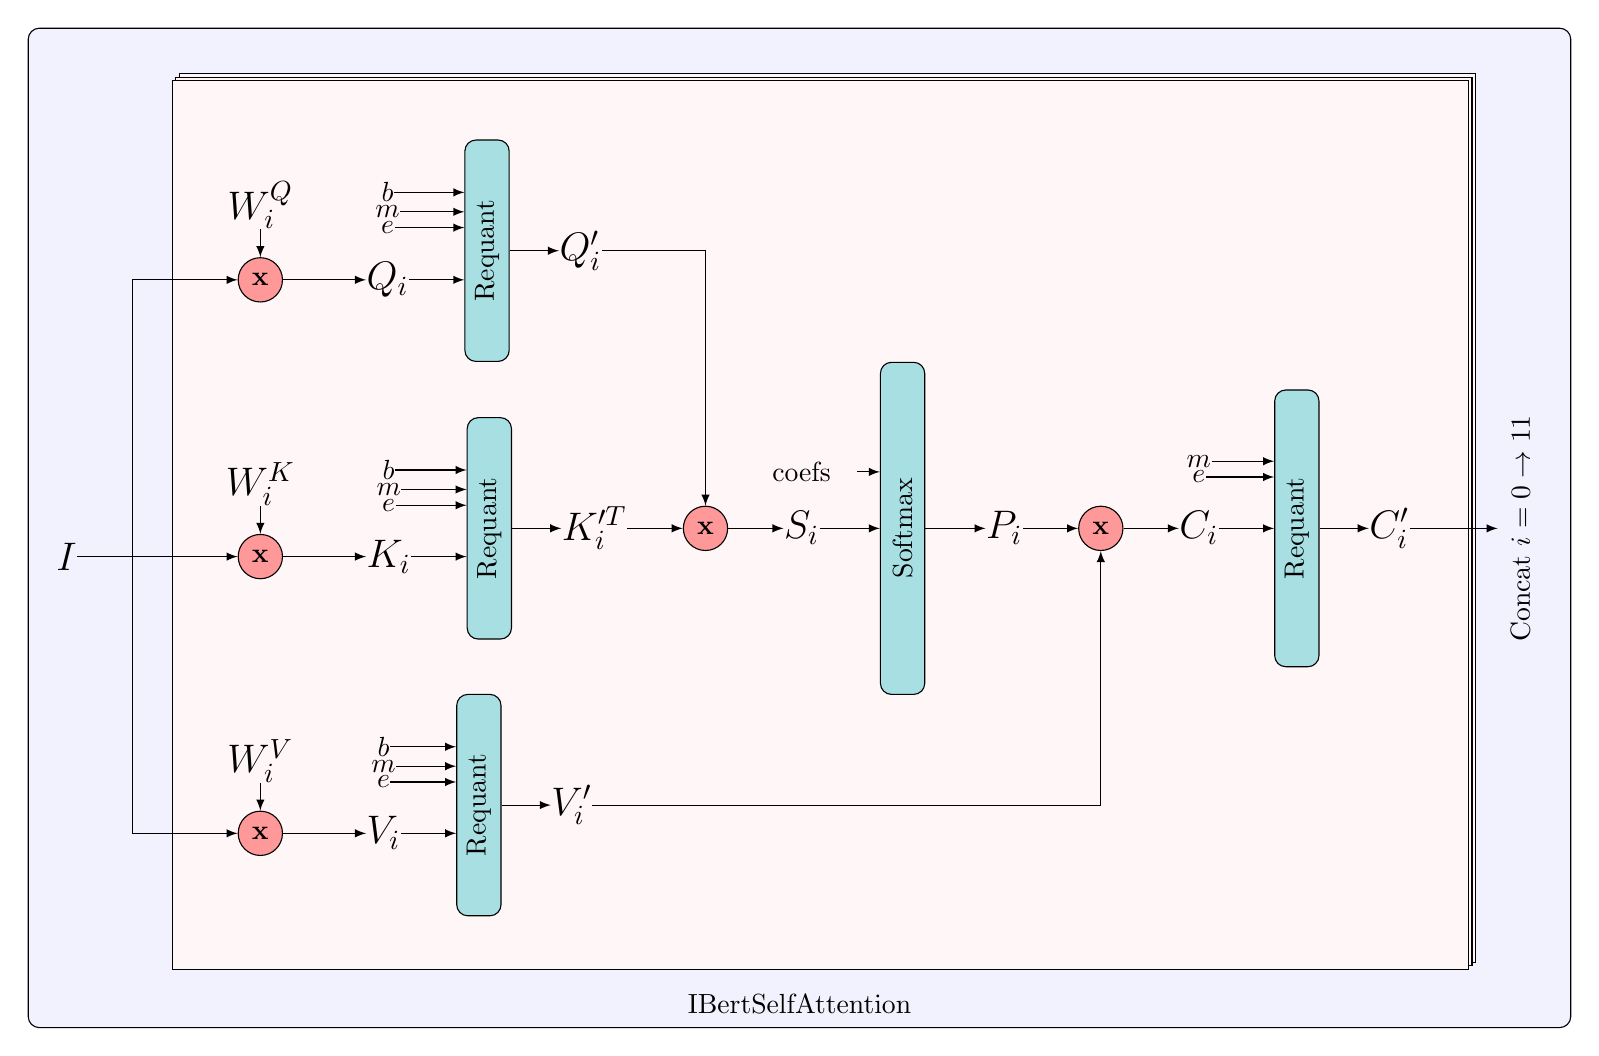
\begin{tikzpicture}[inner sep=0.0 pt, align=center]
    \pgfmathsetmacro{\rectWidth}{40}
    \pgfmathsetmacro{\rectHeight}{40}

    \node (layer_input) [rectangle, draw=none, font=\Large] at (0,0) {$I$};

    \pgfmathsetmacro{\multSize}{16 pt}
    \node [draw, circle, fill=lightRed, minimum size=\multSize, right=\rectWidth*1.75pt of layer_input.center, anchor=center] (mult1) {\textbf{x}};
    \node [draw, circle, fill=lightRed, minimum size=\multSize, above=\rectHeight*2.5pt of mult1.center, anchor=center] (mult2) {\textbf{x}};
    \node [draw, circle, fill=lightRed, minimum size=\multSize, below=\rectHeight*2.5pt of mult1.center, anchor=center] (mult3) {\textbf{x}};

    \node (weight_Q) [rectangle,draw=none,font=\Large,above=\rectHeight*0.25pt of mult2] {$W_i^Q$};
    \node (weight_K) [rectangle,draw=none,font=\Large,above=\rectHeight*0.25pt of mult1] {$W_i^K$};
    \node (weight_V) [rectangle,draw=none,font=\Large,above=\rectHeight*0.25pt of mult3] {$W_i^V$};

    \draw [-latex] (weight_Q.south) -- (mult2.north);
    \draw [-latex] (weight_K.south) -- (mult1.north);
    \draw [-latex] (weight_V.south) -- (mult3.north);

    \draw [-latex] (layer_input.east) -| ([xshift=\rectWidth*0.5 pt]layer_input.east) |- (mult2.west);
    \draw [-latex] (layer_input.east) -| ([xshift=\rectWidth*0.5 pt]layer_input.east) |- (mult1.west);
    \draw [-latex] (layer_input.east) -| ([xshift=\rectWidth*0.5 pt]layer_input.east) |- (mult3.west);

    \node (mixQ32b) [right=\rectWidth*0.75pt of mult2,font=\Large] {$Q_i$};
    \node (mixK32b) [right=\rectWidth*0.75pt of mult1,font=\Large] {$K_i$};
    \node (mixV32b) [right=\rectWidth*0.75pt of mult3,font=\Large] {$V_i$};

    \draw [-latex] (mult2.east) -- (mixQ32b.west);
    \draw [-latex] (mult1.east) -- (mixK32b.west);
    \draw [-latex] (mult3.east) -- (mixV32b.west);

    \node (qreq_e)[rectangle,draw=none,above=\rectHeight*0.25pt of mixQ32b.north] {$e$};
    \node (qreq_m)[rectangle,draw=none,above=1.0pt of qreq_e.north] {$m$};
    \node (qbias) [rectangle,draw=none,above=1.0pt of qreq_m.north] {$b$};
    
    \node (kreq_e)[rectangle,draw=none,above=\rectHeight*0.25pt of mixK32b.north] {$e$};
    \node (kreq_m)[rectangle,draw=none,above=1.0pt of kreq_e.north] {$m$};
    \node (kbias) [rectangle,draw=none,above=1.0pt of kreq_m.north] {$b$};
    
    \node (vreq_e)[rectangle,draw=none,above=\rectHeight*0.25pt of mixV32b.north] {$e$};
    \node (vreq_m)[rectangle,draw=none,above=1.0pt of vreq_e.north] {$m$};
    \node (vbias) [rectangle,draw=none,above=1.0pt of vreq_m.north] {$b$};
    
    \node [draw, fill=lightCyan, rounded corners, minimum width=\rectHeight*2, minimum height=\rectWidth*0.4, rotate=90, above right=\rectWidth*0.1pt and \rectWidth*0.5pt of mixQ32b, anchor=north] (reqQ) {Requant};
    \node [draw, fill=lightCyan, rounded corners, minimum width=\rectHeight*2, minimum height=\rectWidth*0.4, rotate=90, above right=\rectWidth*0.1pt and \rectWidth*0.5pt of mixK32b, anchor=north] (reqK) {Requant};
    \node [draw, fill=lightCyan, rounded corners, minimum width=\rectHeight*2, minimum height=\rectWidth*0.4, rotate=90, above right=\rectWidth*0.1pt and \rectWidth*0.5pt of mixV32b, anchor=north] (reqV) {Requant};

    \draw [-latex] (qreq_e.east) to[out=0,in=180] (reqQ.north |- qreq_e);
    \draw [-latex] (qreq_m.east) to[out=0,in=180] (reqQ.north |- qreq_m);
    \draw [-latex] (qbias.east) to[out=0,in=180] (reqQ.north |- qbias);

    \draw [-latex] (kreq_e.east) to[out=0,in=180] (reqK.north |- kreq_e);
    \draw [-latex] (kreq_m.east) to[out=0,in=180] (reqK.north |- kreq_m);
    \draw [-latex] (kbias.east) to[out=0,in=180] (reqK.north |- kbias);

    \draw [-latex] (vreq_e.east) to[out=0,in=180] (reqV.north |- vreq_e);
    \draw [-latex] (vreq_m.east) to[out=0,in=180] (reqV.north |- vreq_m);
    \draw [-latex] (vbias.east) to[out=0,in=180] (reqV.north |- vbias);
    
    \draw [-latex] (mixQ32b.east) to[out=0,in=180] (reqQ.north |- mixQ32b);
    \draw [-latex] (mixK32b.east) to[out=0,in=180] (reqK.north |- mixK32b);
    \draw [-latex] (mixV32b.east) to[out=0,in=180] (reqV.north |- mixV32b);


    \node (mixQ8b)[right=\rectWidth*0.65pt of reqQ.center,font=\Large]{$Q_i'$};
    \node (mixK8b)[right=\rectWidth*0.65pt of reqK.center,font=\Large]{$K_i'^T$};
    \node (mixV8b)[right=\rectWidth*0.65pt of reqV.center,font=\Large]{$V_i'$};

    \draw [-latex] (reqQ.south) -- (mixQ8b.west);
    \draw [-latex] (reqK.south) -- (mixK8b.west);
    \draw [-latex] (reqV.south) -- (mixV8b.west);

    \node [draw, circle, fill=lightRed, minimum size=\multSize, right=\rectWidth*0.5pt of mixK8b] (multSelf1) {\textbf{x}};
    \node (Si) [right=\rectWidth*0.5pt of multSelf1,font=\Large]{$S_i$};

    \draw [-latex] (mixQ8b.east) -| (multSelf1.north);
    \draw [-latex] (mixK8b.east) -- (multSelf1.west);
    \draw [-latex] (multSelf1.east) -- (Si.west);

    \node [draw=none, rectangle, text width=\rectWidth, minimum width=\rectWidth, minimum height=\rectHeight*0.2, above=\rectHeight*0.25pt of Si.north] (coef) {coefs};

    \node [draw, fill=lightCyan, rounded corners, minimum width=\rectHeight*3, minimum height=\rectWidth*0.4, rotate=90, right=\rectWidth*0.75pt of Si, anchor=center] (softmax) {Softmax};

    \draw [-latex] (coef.east) to[out=0,in=180] (softmax.north |- coef);

    \node (Pi)[right=\rectWidth*0.75pt of softmax.center,font=\Large]{$P_i$};
    \node [draw, circle, fill=lightRed, minimum size=\multSize, right=\rectWidth*0.5pt of Pi] (multSelf2) {\textbf{x}};
    \node (Ci)[right=\rectWidth*0.5pt of multSelf2,font=\Large]{$C_i$};
    \node [draw, fill=lightCyan, rounded corners, minimum width=\rectHeight*2.5, minimum height=\rectWidth*0.4, rotate=90, right=\rectWidth*0.5pt of Ci, anchor=north] (reqC) {Requant};
    \node (Ci8b)[right=\rectWidth*0.65pt of reqC.center,font=\Large]{$C_i'$};

    % \node [draw, rectangle, fill=lightGreen, font=\footnotesize, text width=\rectWidth, minimum width=\rectWidth, minimum height=\rectHeight*0.2, above=\rectHeight*0.25pt of Ci.north] (creq_e) {$e$};
    % \node [draw, rectangle, fill=lightGreen, font=\footnotesize, text width=\rectWidth, minimum width=\rectWidth, minimum height=\rectHeight*0.2, above=1.0pt of creq_e.north] (creq_m) {$m$};

    \node (creq_e)[above=\rectHeight*0.25pt of Ci.north]{$e$};
    \node (creq_m)[above=1.0pt of creq_e.north]{$m$};

    \draw [-latex] (creq_e.east) to[out=0,in=180] (reqC.north |- creq_e);
    \draw [-latex] (creq_m.east) to[out=0,in=180] (reqC.north |- creq_m);
    % \draw [-latex] (Ci.east) to[out=0,in=180] (reqC.north |- Ci);

    \draw [-latex] (Si.east) -- (softmax.north);
    \draw [-latex] (softmax.south) -- (Pi.west);
    \draw [-latex] (Pi.east) -- (multSelf2.west);
    
    \draw [-latex] (mixV8b.east) -| (multSelf2.south);
    \draw [-latex] (multSelf2.east) -- (Ci.west);
    \draw [-latex] (reqC.south) -- (Ci8b.west);
    \draw [-latex] (Ci.east) -- (reqC.north);

    \begin{pgfonlayer}{main_bg}
        \node (self_rect) [draw, rectangle, fill=black!3, inner sep=20pt, fit=(weight_Q)(weight_K)(weight_V)(mixQ32b)(mixV32b)(Ci8b)(reqQ)(reqK)(reqV)] {};
        \begin{pgfonlayer}{back_bg}
            \foreach \x in {3,...,1} {
                \node [draw, rectangle, fill=red!3, fit=(self_rect), above right=\x*1.25pt-\the\pgflinewidth and \x*1.25pt-\the\pgflinewidth of self_rect.south west] {};
            }
        \end{pgfonlayer}
    \end{pgfonlayer}

    \node [draw=none, minimum width=\rectHeight*3, minimum
      height=\rectWidth*0.4, rotate=90, right=\rectWidth*1pt of Ci8b,
    anchor=center] (concat) {Concat $i=0\rightarrow11$};
    \draw [-latex] (Ci8b.east) -- (concat.north);

    \begin{pgfonlayer}{main_bg}
        % fill=red!3
        \node (SelfAtt) [draw, rectangle, fill=blue!5, rounded corners, inner xsep=10pt, inner ysep=20pt, fit=(layer_input)(self_rect)(concat)] {};
        \node (SelfAttText) [above=5.0pt of SelfAtt.south] {IBertSelfAttention};

        % \node (all) [draw, rectangle, inner xsep=20pt, inner ysep=40pt, fit=(layer_input)(weight_Q)(weight_K)(weight_V)(mixQ32b)(mixV32b)(Ci8b)(concat)] {};
    \end{pgfonlayer}


    \end{tikzpicture}

\end{document}
